
\section{Discovery and Integration}
\label{sec:application}

\begin{figure*}[!t]
\centering
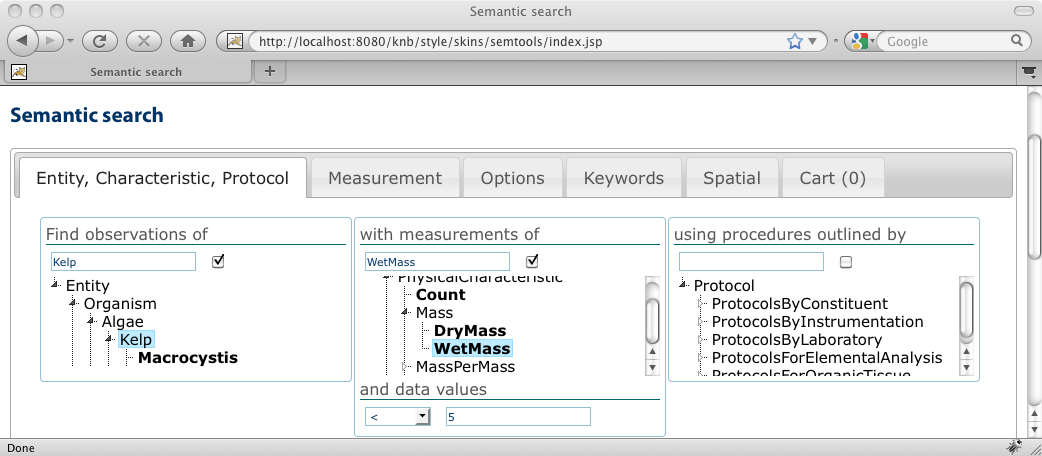
\includegraphics[width=1.0\textwidth]{images/metacat-query.png}
\caption{Semantic data query web interface. Data packages containing observations of Kelp Wet Mass less than or equal to 5 [grams] are returned. Additional search options and compound query criteria can be specified within the other tabs. Matches can be saved in the data cart for later exploration.}
\label{fig:metacat-query}
\end{figure*}

\mypara{Concept query.} The semantic query interface primarily supports locating datasets by how well their observational models match the given criteria. Query criteria largely mirror the structure of an Annotation in that combinations of Entity, Characteristic and Protocol are specified and optionally compounded when increased precision is sought. 

By leveraging the relationships defined and/or inferred from the
ontology we are able to increase recall beyond what is possible for
simple keyword-based searches
\cite{berkley09:_improv_data_discov_for_metad}. Broad queries return
direct matches and also n-depth subclass matches. The queries can be
quickly honed when using this browsing paradigm which allows rapid
exploration of the data repository without the oneous of defining
complete observational queries \emph{de novo}. Measurement ``templates''
as defined in OBOE compatible ontologies enable a single concept to
proxy its constituent parts, namely the characteristics of
particular entities that can be measured with a set of protocols and
standards. This short-hand query generation highlights a
compelling reason for using OBOE extension ontologies and can
also be leveraged when creating or editing semantic annotations in the Morpho interface.  

Using compound semantic query criteria applies a finer-grained filter on the datasets that are
returned. Results can be restricted to only those datasets that include 
measurements for a set of specific characteristics of a particular
observational entity. Furthermore, a query can specify that those measurements come
from precisely the \emph{same instance of that entity}; a feature that fully exercises the comprensive observational structure expressed in the annotation.

\mypara{Data query.} For even more precise recall, the OBOE model can be partially \emph{materialized} during the query stage after which a data range filter can be applied. Different techniques are available for merging the annotation with the data that it describes, but for performance reasons a hybrid approach has been adopted in which premliminary search results from a concept query are collated and only that subset is materialized. Because our corpus is described using EML in conjunction with the annotation syntax, the Data Manager Library can handily load the described raw data while the annotation informs the correct use of the Data Manager query and filtering features. For any measurements that match the concept query criteria, we verify that those measurements (e.g., attributes) contain data values within the range specifed in the initial semantic data query and return the data packages that contain them (\figref{fig:metacat-query}).

\mypara{Data integration.} The materialization routine used for semantic data queries laid the groundwork for our ongoing data integration pursuits. In addition to inspecting the data for values within a range and returning the datasets that contain a match, the ``smart'' data integration feature goes further by constructing a synthetic data product that represents the complete results of the query in terms of both the attributes and the values that are returned. Each original data object may have wildly different syntactic structures (e.g. column number, naming, order) but could share a subset of attributes that are semantically compatible as defined in accompanying annotations. These compatible, in-common attributes become the facets and metrics in a synthetic dataset; their values filtered accordingly (\figref{fig:integration}). While preliminary results have been quite promising - albeit academic - continued development of algorithms for determining compatibility of annotated measurements (e.g., gram and ounce are both mass units) and for mutating measurement values using ontologically-defined conversions (e.g., 1000 milligrams in a gram) will enable increasingly thorough, automated data integration practices.


\begin{figure}
\centering
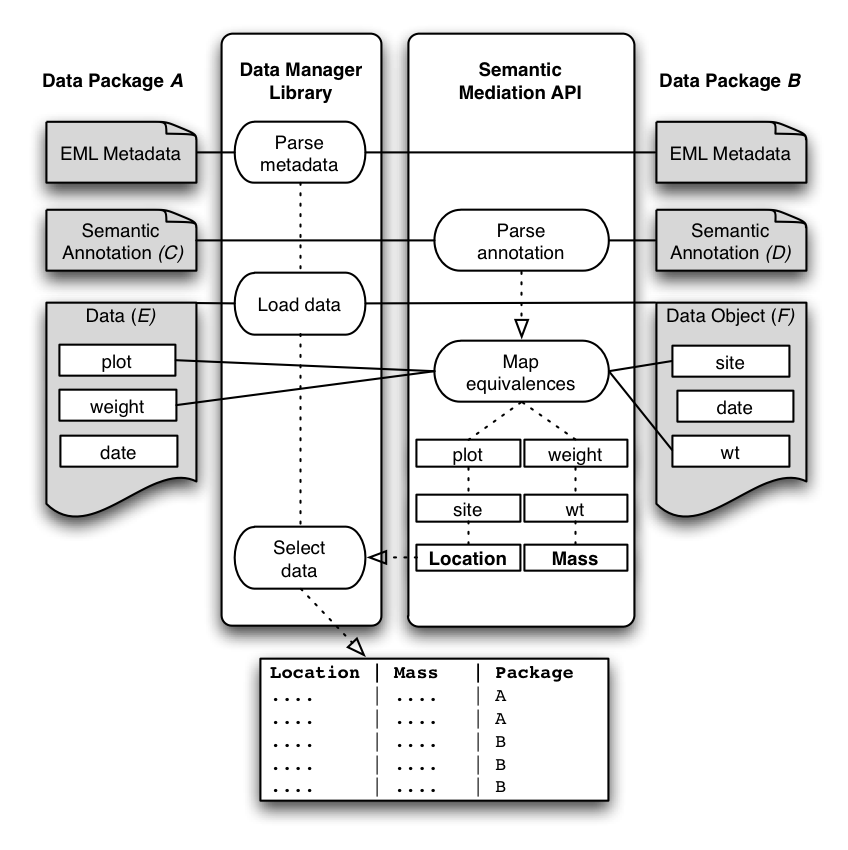
\includegraphics[scale=1.0]{images/integration.png}
\caption{Data integration query across multiple data packages (A, B).  Annotations (C, D) are used to determine semantically equivalent data attributes contained in the data objects (E, F). Attributes 'plot' and 'site' are considered equivalent measurements of the characteristic 'Location'; attributes 'weight' and 'wt' both map to the same characteristic 'Mass'. The Semantic Mediation API utilizes the Data Manager Library to load and query the source data informed by semantic similarities between the structurally disparate data attributes.}
\label{fig:integration}
\end{figure}

%%% Local Variables: 
%%% mode: latex
%%% TeX-master: "main"
%%% End: 
